%%%%%%%%%%%%%%%%%%%%%%%%%%%%%%%%%%%%%%%%%%%%%%%%%%%%%%%%%%%%%%%%%%%%%%%%%%%%%%%%%%%%%
% Fundamental Current i^1_1 and fundamental volage u^1_2 for single-phase DC inverter
%%%%%%%%%%%%%%%%%%%%%%%%%%%%%%%%%%%%%%%%%%%%%%%%%%%%%%%%%%%%%%%%%%%%%%%%%%%%%%%%%%%%%
\begin{figure}[htb]

    %   \documentclass{standalone}
    %   \usepackage{pgfplots}
    %   \pgfplotsset{compat=1.18} % Kompatibilität für neuere Versionen
           \centering
           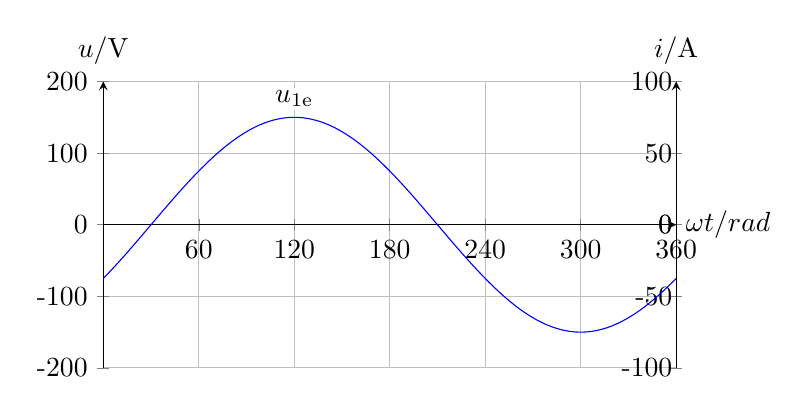
\begin{tikzpicture}
                \pgfplotsset{set layers}
           \begin{axis}[
            % x/y range adjustment
            scale only axis,
            ymin=-200, ymax=200,
            xmin=0, xmax=360, 
            samples=500,
            axis y line=center,
            axis x line=middle,
            extra y ticks=0,
            % Label text
            xlabel={$\omega t / \text{rad}$},
            ylabel={$u/\mathrm{V}$},
            % Label adjustment
            x label style={at={(axis description cs:1,0.5)},anchor=west},
            y label style={at={(axis description cs:0,.97)},anchor=south,yshift=0.2cm},
            width=0.6\textwidth,
            height=0.3\textwidth,
            % x-Ticks
            xtick={0,60,120,180,240, 300, 360},
            xticklabels={0,60,120,180,240, 300, 360},
            xticklabel style = {anchor=north},
            % y-Ticks
            ytick={-200,-100,0,100,200},
            yticklabels={-200,-100,0,100,200},
            yticklabel style = {anchor=east},
            % Grid layout
            grid,
            %grid style={line width=.1pt, draw=gray!10},
            %major grid style={line width=.2pt,draw=gray!90},
        ] 
        % internal load voltage u
        \addplot[blue, domain= 0:360, solid] {150*sin(x-(180/6))};
         % Label of u
         \node[black, fill=white, inner sep = 1pt, anchor = south] at (axis cs:120,160) {$u_\mathrm{1e}$};
           \end{axis}
           \begin{axis}[
            % x/y range adjustment
            scale only axis,
            ymin=-100, ymax=100,
            xmin=0, xmax=360,
            axis x line=none, 
            samples=500,
            axis y line=right,
            axis x line=middle,
            extra y ticks=0,
            % Label text
            ylabel={$i/\mathrm{A}$},
            % Label adjustment
            y label style={rotate = -90,at={(axis description cs:1,.97)},anchor=south,yshift=0.2cm},
            width=0.6\textwidth,
            height=0.3\textwidth,
            % y-Ticks
            ytick={-100,-50,0,50,100},
            yticklabels={-100,-50,0,50,100},
            yticklabel style = {anchor=east},
            % Grid layout
            grid,
            %grid style={line width=.1pt, draw=gray!10},
            %major grid style={line width=.2pt,draw=gray!90},
        ]
           \end{axis}             
           \end{tikzpicture}
           \caption{Internal load voltage $u_\mathrm{1e}$, fundamental voltage and current components $u^\mathrm{(1)}_\mathrm{2}(t)$
            and  $i^\mathrm{(1)}_\mathrm{2}(t)$, respectively. }
           \label{sfig:ex07_sub1.2_fund_components}
   \end{figure}